
A continuación se muestran los casos de uso para los oficios salientes.
\begin{figure}[htbp!]
		\centering
			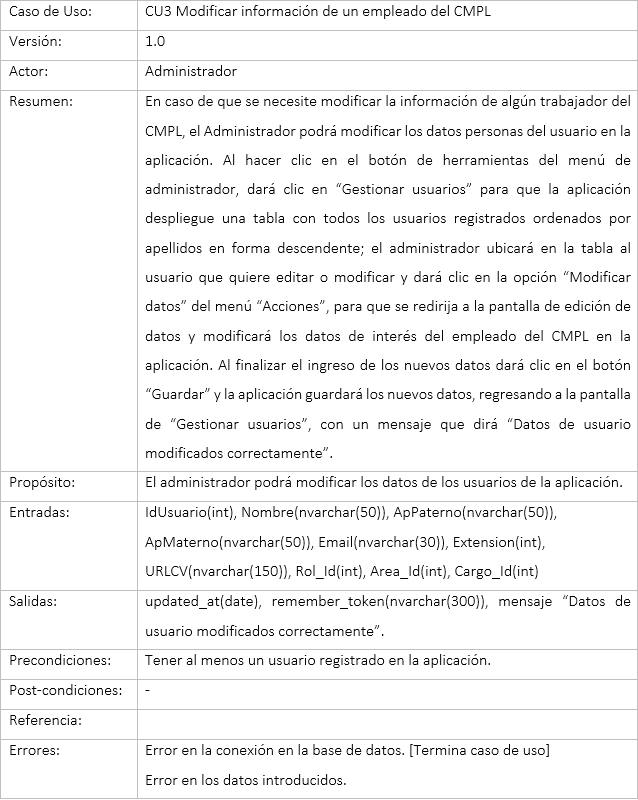
\includegraphics[width=0.8\textwidth]{images/CU/CU3}
		\caption{Caso de Uso 3 Registrar oficio saliente.}
		\label{diagrama a bloques}
	\end{figure}

\begin{itemize}
	\item Trayectoria principal:
	\begin{enumerate}
		\item El actor va a la sección de correspondencia 
		\item La aplicación muestra la pantalla IU4 Correspondencia.
		\item El actor presiona el botón “Nuevo oficio”.
		\item La aplicación muestra la interfaz IU4.1 para el registro de oficios.
		\item El actor introduce los datos requeridos para el registro del oficio.
		\item El actor presiona el botón “Adjuntar documento”.
		\item CU27 Guardar Archivo.
		\item El usuario presiona el botón “Registrar”. 
		\item La aplicación hace la validación de los datos introducidos. [Trayectoria alternativa A] 
		\item La aplicación muestra el mensaje MSG2 de que el registro se realizó de forma exitosa.
		\item Fin del caso de uso.
	\end{enumerate}
	
	\item Trayectorias alternativas:
	\begin{itemize}
		\item Trayectoria alternativa A:
			\begin{enumerate}
				\item La aplicación muestra un mensaje de error.
				\item La aplicación resalta los campos en el formulario con errores.
				\item El usuario corrige los errores en el formulario.
				\item Continua en trayectoria del CU3 en paso 8.
			\end{enumerate}
	\end{itemize}
\end{itemize}

